\documentclass[12pt]{article}
\usepackage{fullpage,graphicx,psfrag,amsmath,amsfonts,verbatim}
\usepackage[small,bf]{caption}
\usepackage{epstopdf}
\usepackage{epsfig}
\usepackage{setspace}
\usepackage{amsthm}
\usepackage{algorithm}
\usepackage{algorithmic}
\usepackage{tikz}

%\doublespacing


\def\E{\mathbb{E}}
\def\P{\mathbb{P}}
\def\R{\mathbb{R}}
\def\G{\mathcal{G}}
\def\N{\mathbb{N}}
\def\Abf{\mathbf{A}}
\def\Psibf{\bm{\Psi}}
\def\Ibf{\mathbf{I}}
\def\fbf{\mathbf{f}}
\def\xbf{\mathbf{x}}
\def\ybf{\mathbf{y}}
\def\zbf{\mathbf{z}}
\def\nbf{\mathbf{n}}
\def\ubf{\mathbf{u}}
\def\pbf{\mathbf{p}}
\def\p{\mathbf{\pi}}
\def\sbf{\mathbf{s}}
\def\rbf{\mathbf{r}}
\def\vbf{\mathbf{v}}
\def\taubf{\bm{\tau}}
\def\Wbf{\mathbf{W}}
\def\1{\mathbf{1}}
% Indicator function
\def\indfcn{\mathbbm{1}}

\def\N{\mathbb{N}}
\def\MM{\mathcal{M}}
\def\RR{\mathcal{R}}
\def\AA{\mathcal{A}}


\def\d{\overline{d}}
\def\dd{\underline{d}}

\def\T{\overline{T}}
\def\TT{\underline{T}}

% argmin and argmax operators
\newcommand{\argmin}[1]{{\underset{#1}{\operatorname{argmin}}}}
\newcommand{\argmax}[1]{{\underset{#1}{\operatorname{argmax}}}}



\newtheorem{theorem}{Theorem}
\newtheorem{lemma}[theorem]{Lemma}
\newtheorem{proposition}[theorem]{Proposition}
\newtheorem{corollary}[theorem]{Corollary}
\newtheorem{definition}{Definition}
\newtheorem{assumption}{Assumption}

\bibliographystyle{alpha}

\title{Bandit Algorithm for Multiple Hypothesis Testing}
\author{}
\date{}
\begin{document}
\maketitle


\section{Problem Formulation}
Consider an agent who has a set $\MM = \{1,2,\cdots,m\}$ of different options (arms) with the unknown mean values $\{\mu_1,\mu_2,\cdots,\mu_m\}$. At any time step $t\in\N$, the agent observes a new data point $X^t_i$ for any arm $i$ which is generated according to
\begin{equation}
\label{model1}
X^t_i = \mu_i + n^t_i,
\end{equation}
where $n^t_i$ is zero mean noise components associated to arm $i$ at time $t$. The noise components are independent across different arms $i = 1,2,\cdots,m$ and iid distributed across different time steps $t \in\N$ for any arm $i$. The agent's goal is to identify which  arms are {\em close} in performance to a base arm-- called arm 0-- and which arms are {\em different} from the base arm in a sequential manner. The base arm has a mean value of $\mu_0$ and for a given sensitivity level $\epsilon>0$, arm $i$ is considered close to the base arm if $|\mu_0-\mu_i|< \epsilon$ and different from the base arm if $|\mu_0-\mu_i|>\epsilon$. 
Specifically, the agent wants to develop an algorithm which, at any time $t\in\N$ and  based on the observed data $\{X_i^1,X_i^2,\cdots,X_i^t\}$ for any arm $i\in\MM$, makes one of the following decisions for arm $i$: 
\begin{enumerate}
\item confidently accepts the null hypothesis $H_0^i:|\mu_i-\mu_0|< \epsilon$ against the alternative hypothesis $H^i_1:|\mu_i-\mu_0|> \epsilon$,
\item confidently rejects the null hypothesis $H_0^i:|\mu_i-\mu_0|< \epsilon$ against the alternative hypothesis $H^i_1:|\mu_i-\mu_0|> \epsilon$,
\item waits for more observations of arm $i$.
\end{enumerate}
The agent stops running the algorithm once all the null hypotheses are either accepted or rejected.

For such an algorithm, let  $\RR$ and $\AA$ be the set of rejected and accepted null hypotheses returned at the stopping time, respectively.  Also, let $\MM_r = \{i\in\MM:|\mu_i-\mu_0|>\epsilon\}$ and $\MM_a = \{i\in\MM:|\mu_i-\mu_0|<\epsilon\}$ be the set of $\epsilon$-different and  $\epsilon$-equal arms to the base arm, respectively. For the problem to be well-defined, we assume that there is no arm with a mean value $\mu_0+\epsilon$ or $\mu_0-\epsilon$.  Furthermore, let $R,A,m_r$ and $m_a = m-m_r$, denote the size of the sets $\RR,\AA,\MM_r$ and $\MM_a$, respectively. Now, define  $V= |\MM_a\cap\RR|$ as  the number of false negatives (number of incorrectly rejected arms) and $W = |\MM_r\cap\AA|$ be as the number of false positives (number of incorrectly accepted arms) by the the algorithm. The type I and type II Family-Wise Error Rate (FWER) of the algorithm are then defined as 
$$E_1 = \P[V\geq 1],~~~~ E_2 = \P[W\geq 1],$$
respectively. Table \ref{table1} summarizes the relations among different parameters defined above. 
\begin{table}[t]
\begin{center}
\begin{tabular}{c|c|c|c}
&accepted&rejected&total\\
\hline
$H_0$ true&$m_a-V$&\textbf{$V$}&$m_a$\\
$H_0$ false&$W$&$m_r-W$&$m_r$\\
\hline
total& $A$&$R$&$m$
\end{tabular}
\end{center}
\caption{Various Parameters in Multiple Hypothesis Testing}\label{table_multi}
\label{table1}
\end{table}

The agent's goal is to design a sequential hypotheses testing algorithm which guarantees the following FWER  bounds
$$
 E_1\leq \alpha,~~~~E_2\leq \beta,
$$
for any given value of $\alpha,\beta\in (0,1)$. 

\section{The Bandit Algorithm}
We now propose a bandit algorithm for the above hypothesis testing problem. First, we focus on the scenario in which the performance of the base arm (i.e., $\mu_0$) is known to the agent. Later, we describe how we can modify our proposed algorithm to relax this assumption. Furthermore, we make the following assumption on the tail of the noise components in \eqref{model1}. 
\begin{assumption}
\label{assmp1}
There exists $\sigma>0$ such that the noise component $n^t_i$ is  $\frac{\sigma^2}{4}$-subgaussian for all $i,t$.
\end{assumption}
For example, if $X^t_i$ is a Binary random variables for all $i,t$, then we meet 
Assumption \ref{assmp1} by taking $\sigma^2 = 1$. Furthermore, if there 
exists, $a_i,b_i$ for each $i$ such that $X^t_i\in [a_i,b_i]$ almost surely for all  $t\in\N$, then $n^t_i$ is $(b_i-a_i)^2$-subgaussian for any $t$  and 
hence, taking $\sigma^2 = \max_{i}~(b_i-a_i)^2$ will satisfy Assumption~\ref{assmp1}. 



\begin{algorithm}[tb]
   \caption{Bandit Multiple Hypothesis Testing}
   \label{alg1}
\begin{algorithmic}
   \STATE {\bfseries Input:} $\MM,\mu_0,\epsilon,\alpha,\beta,\{\Delta_t\}_{t\in\mathbb{N}}$
   \STATE{\bfseries Initialize:} $t=1$ and $M_t = \MM$
   \WHILE{$M_t$ is non-empty }
   \STATE pull each arm $i\in M_t$ once and observe the data
   \STATE Compute empirical means $\hat\mu^t_i,~\forall~i\in M_t$
  \FOR{$i \in M_t$}
  	\IF{$|\hat\mu_i^t - \mu_0|>\big(\epsilon+\Delta_t(\alpha)\big)$}
  		\STATE {\bf Reject} $H_0^i$
  		\STATE Remove $i$ from $M_t$ and add it to $\RR$
  	\ENDIF
  	
  \IF{$|\hat\mu_i^t - \mu_0|<\big(\epsilon-\Delta_t(\beta)\big)$}
  		\STATE {\bf Accept} $H_0^i$
  		\STATE Remove $i$ from $M_t$ and add it to $\AA$
  	\ENDIF
  \ENDFOR
  \STATE $t \leftarrow t+1$
   \ENDWHILE
   
\end{algorithmic}
\end{algorithm} 



Our proposed algorithm --described in Algorithm \ref{alg1}-- takes as input the set of arms $\MM$, mean value of the base arm $\mu_0$, $\epsilon$, desired  errors $\alpha, \beta$ and a sequence of concentration functions $\Big\{\Delta_t:(0,1)\to\mathbb{R}\Big\}_{t\in\mathbb{N}}$ which for any $x\in(0,1)$ satisfies 
\begin{equation}
\label{Delta1}
\P\big[|\mu_i-\hat\mu_i^t|\leq\Delta_t(x),~\forall~i\in\MM,t\in \mathbb{N}\big]\geq 1-x,
\end{equation}
where $\hat\mu_i^t$ is the empirical mean of arm $i$ at time $t$. 
One standard choice for $\Delta$ is the error bound of Hoeffding inequality combined with a union bound over all arms and all time steps; i.e., 
\begin{equation}
\label{hofDelta}
\Delta_t(x) = \sqrt{\frac{\sigma^2}{2t}\log\Big(\frac{4mt^2}{x}\Big)}.
\end{equation}
The following proposition shows that this sequence of $\Delta_t$ satisfies \eqref{Delta1}. 
\begin{proposition}
With $\Delta_t$ given in \eqref{hofDelta}, we have
$$\P\big[|\mu_i-\hat\mu_i^t|\leq\Delta_t(x),~\forall~i\in\MM,t\in \mathbb{N}\big]\geq 1-x,$$
for any $x\in(0,1)$.
\end{proposition}
\begin{proof}

First note that for any $x\in(0,1)$, we have
$$\begin{aligned}
\P\big[\exists i\in\MM,t\in\N: |\mu_i - \hat\mu^t_i|>\Delta_t(x)\big] &\stackrel{\text{(a)}}{ \leq} \sum_{i=1}^m \sum_{t=1}^\infty \P\big[ |\mu_i - \hat\mu^t_i|>\Delta_t(x)\big]\\
&\stackrel{\text{(b)}}{\leq}  \sum_{i=1}^m \sum_{t=1}^\infty 2\exp\bigg(-\frac{2t\Delta_t(x)^2}{\sigma^2}\bigg),
\end{aligned}$$
where {\bf (a)} follows from a union bound and {\bf (b)} is an application of Hoeffding bound for $\frac{\sigma^2}{4}$-subgaussian random variables. Substituting from \eqref{hofDelta} for $\Delta_t(x)$ in the above equation gives
$$
\begin{aligned}
\P\big[|\mu_i-\hat\mu_i^t|\leq\Delta_t(x),~\forall~i\in\MM,t\in \mathbb{N}\big] & = 1- \P\big[\exists i\in\MM,t\in\N: |\mu_i - \hat\mu^t_i|>\Delta_t(x)\big]\\
&\geq 1- \sum_{i=1}^m \sum_{t=1}^\infty 2 \exp\bigg(-\frac{2t}{\sigma^2}\frac{\sigma^2}{2t}\log\Big(\frac{4mt^2}{x}\Big)\bigg)\\
&= 1 - \sum_{i=1}^m \sum_{t=1}^\infty 2 \frac{x}{4mt^2} \\
& = 1 - \frac{x}{2}\sum_{t=1}^\infty \frac{1}{t^2} \\
& = 1 -  \frac{x}{2}\frac{\pi^2}{6}\\
& \geq 1 - x.
\end{aligned}$$
\end{proof}

Figure \ref{fig1}  summarizes the nature of the proposed bandit algorithm. At any time $t$, three different regions ("rejection", "acceptance" and "no decision") are recognized and a decision is made for each arm based on the region its empirical mean lies in. 

\begin{algorithm}[tb]
   \caption{Bernstein Multiple Hypothesis Testing}
   \label{alg4}
\begin{algorithmic}
   \STATE {\bfseries Input:} $\MM,\mu_0,\epsilon,\alpha,\beta,R$
   \STATE{\bfseries Initialize:} $t=1$ and $M_t = \MM$
   \WHILE{$M_t$ is non-empty }
   \STATE pull each arm $i\in M_t$ once and observe the data
   \STATE Compute empirical means $\hat\mu^t_i,~\forall~i\in M_t$
   \STATE Compute empirical standard deviations $,\hat\nu^t_i,~\forall~i\in M_t$
   \STATE Compute $Delta^i_t,~\forall~i\in M_t$ according to \eqref{berndelta}
  \FOR{$i \in M_t$}
  	\IF{$|\hat\mu_i^t - \hat\mu_0^t|>\big(\epsilon+ \Delta^i_t(\alpha)\big)$}
  		\STATE {\bf Reject} $H_0^i$
  		\STATE Remove $i$ from $M_t$ and add it to $\RR$
  	\ENDIF
  	
  \IF{$|\hat\mu_i^t - \hat\mu^t_0|<\Big(\epsilon-\Delta^i_t(\beta)\Big)$}
  		\STATE {\bf Accept} $H_0^i$
  		\STATE Remove $i$ from $M_t$ and add it to $\AA$
  	\ENDIF
  \ENDFOR
  \STATE $t \leftarrow t+1$
   \ENDWHILE
   
\end{algorithmic}
\end{algorithm} 


The  Hoeffding-based sequence $\Delta_t$ defined in \eqref{hofDelta} does not take the variance of each arm into account. In the scenarios where the variance of an arm is very small compared to the range of the possible observations, it is very helpful to use a variance dependent concentration bound, such as the Bernstein inequality. This includes for example, a binary multiple hypothesis testing where we know a priori that the conversion rates are very smaller than 1. Therefore in the scenarios where $X_i^t\in[0,R]$ for some $R\geq 0$ and $Var(X_i^t)\ll R$, we suggest running the proposed algorithm with the following arm-dependent sequence:
\begin{equation}
\label{berndelta}
\Delta_t^i(x) = \hat\nu_i^t\sqrt{\frac{2}{t}\log\Big(\frac{6mt^2}{x}\Big)} + \frac{3R}{t}\log\Big(\frac{6mt^2}{x}\Big),
\end{equation}
where $\hat\nu^t_i$ is the empirical standard deviation of arm $i$ at time $t$ computed as 
\begin{equation}
\label{nu1}
\hat\nu^t_i = \sqrt{\frac{1}{t}\sum_{\tau = 1}^t\big(X^t_i - \hat\mu_i^t\big)^2}.
\end{equation}
Successive steps and details of the algorithm with the above choice of $\Delta$ are summarized in Algorithm \ref{alg4}. While a similar analysis of our proposed algorithm can be carried out with this choice of concentration function, we specialize our analysis in the following section to the Hoeffding-based sequence $\{\Delta_t\}$ defined in \eqref{hofDelta}.


\begin{figure}[t]
\centering
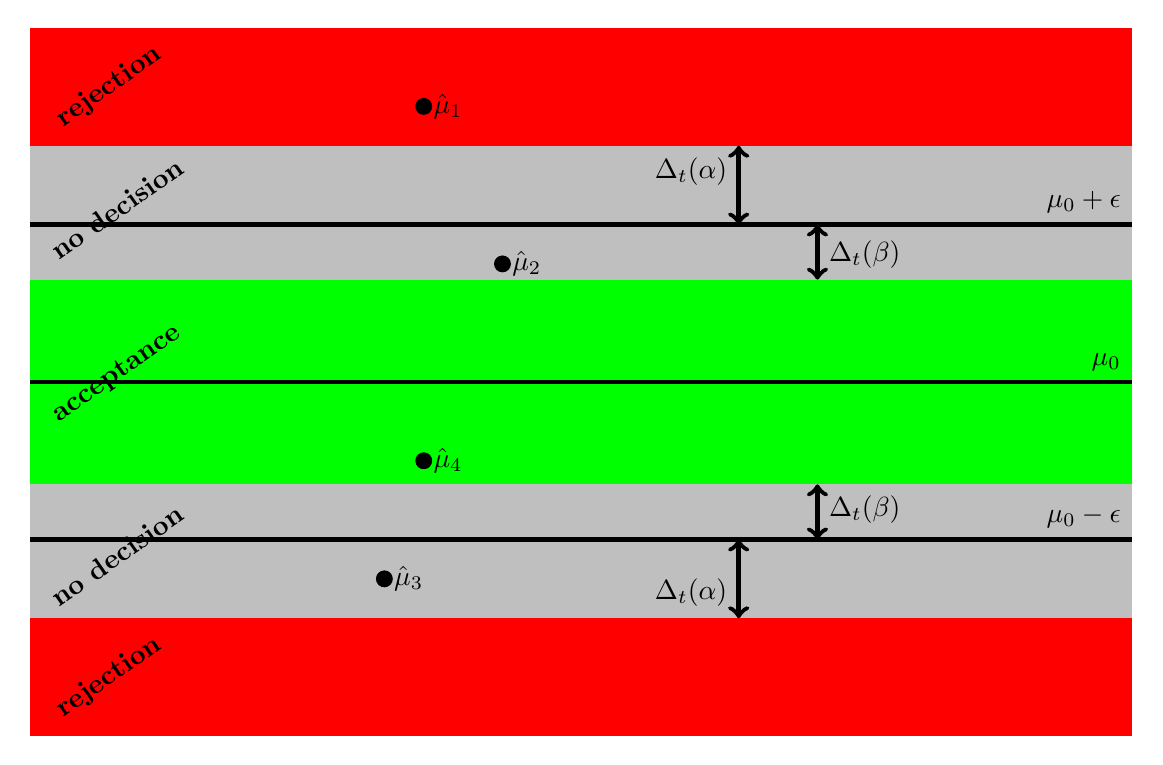
\begin{tikzpicture}
\fill[gray!50] (0,-3) -- (14,-3) -- (14,-1.3) -- (0,-1.3) -- cycle;
\fill[gray!50] (0,3) -- (14,3) -- (14,1.3) -- (0,1.3) -- cycle;
\fill[green!100] (0,-1.3) -- (14,-1.3) -- (14,1.3) -- (0,1.3) -- cycle;
\fill[red!100] (0,-3) -- (14,-3) -- (14,-4.5) -- (0,-4.5) -- cycle;
\fill[red!100] (0,3) -- (14,3) -- (14,4.5) -- (0,4.5) -- cycle;
\draw [line width=0.6mm](0,0) -- (14,0) node[anchor=south east]{ $\mu_0$};
\draw[line width=0.6mm] (0,2)-- (14,2) node[anchor=south east]{$\mu_0+\epsilon$};
\draw [line width=0.6mm](0,-2)--(14,-2) node[anchor=south east]{$\mu_0-\epsilon$};
\draw [fill] (5,-1)  circle (0.1cm) node[anchor= west] {$\hat\mu_4$};
\draw [fill] (6,1.5)  circle (0.1cm) node[anchor= west] {$\hat\mu_2$};
\draw [fill] (5,3.5)  circle (0.1cm) node[anchor= west] {$\hat\mu_1$};
\draw [fill] (4.5,-2.5)  circle (0.1cm) node[anchor= west] {$\hat\mu_3$};
\draw[thick,<->,line width=0.6mm] (10,2) -- (10,1.3) node[anchor=south west]{$\Delta_t(\beta)$};
\draw[thick,<->,line width=0.6mm] (10,-2) -- (10,-1.3) node[anchor=north west]{$\Delta_t(\beta)$};
\draw[thick,<->,line width=0.6mm] (9,2) -- (9,3) node[anchor=north east]{$\Delta_t(\alpha)$};
\draw[thick,<->,line width=0.6mm] (9,-2) -- (9,-3) node[anchor=south east]{$\Delta_t(\alpha)$};
  \node[rotate=35] at 
 (1,3.75)  {{\bf rejection}};
\node[rotate=35] at 
 (1.1,2.2)   {{\bf no decision}};
\node[rotate=35] at 
 (1.1,0.1) {{\bf acceptance}};
 \node[rotate=35] at 
 (1,-3.75)  {{\bf rejection}};
\node[rotate=35] at 
 (1.1,-2.2)   {{\bf no decision}};\end{tikzpicture}
\caption{Different regions recognized by the bandit algorithm at time $t$. At this time, $H_0^1$ is rejected, $H_0^4$ is accepted and no decision has been made for $H_0^2$ and $H_0^3$.}
\label{fig1}
\end{figure}


\section{Analysis}
In this section, we analyze the performance of the proposed bandit algorithm and show that it can guarantee the desired type I and type II errors. Furthermore, we derive an upper bound on the run time of the algorithm. 




\subsection{FWER of the Algorithm}
We start by driving an upper bound on the type I error of the bandit algorithm. We have
\begin{equation}
\label{analysis1}
\begin{aligned}
E_1 &= \P[V \geq 1]\\
& = \P\big[\RR\cap\MM_a~\mbox{is non-empty}\big]\\
& = \P\Big[\exists~i\in\MM_a,t\in\mathbb{N}: ~~\big| \hat\mu^t_i - \mu_0\big|>\big(\epsilon+ \Delta_t(\alpha)\big)\Big]\\
&\stackrel{\text{(a)}}{\leq} \P\Big[\exists~i\in\MM_a,t\in\mathbb{N}: ~~\big| \hat\mu^t_i - \mu_i\big|>\Delta_t(\alpha)\Big]\\
& = 1 - \P\Big[\big| \hat\mu^t_i - \mu_i\big|\leq\Delta_t(\alpha),\forall~i\in\MM_a,t\in\mathbb{N}\Big]\\
&\leq 1 - \P\Big[\big| \hat\mu^t_i - \mu_i\big|\leq\Delta_t(\alpha),\forall~i\in\MM,t\in\mathbb{N}\Big]\\
&\stackrel{\text{(b)}}{\leq}\alpha,
\end{aligned}
\end{equation}
where {\bf (a)} follows because the event $\Big [\exists~i\in\MM_a,t\in\mathbb{N}: ~~\big| \hat\mu^t_i - \mu_i\big|>\big(\epsilon+ \Delta_t(\alpha)\big)\Big]$ implies the event $\Big[\exists~i\in\MM_a,t\in\mathbb{N}: ~~\big| \hat\mu^t_i - \mu_i\big|>\Delta_t(\alpha)\Big] $, and {\bf (b)} follows from \eqref{Delta1}. Therefore, the proposed bandit algorithm guarantees the desired type I FWER. 

To derive type II error rate of the bandit algorithm, we have
\begin{equation}
\label{analysis2}
\begin{aligned}
E_2 &= \P[W\geq 1]\\
& = \P\big[\AA\cap\MM_r~\mbox{is non-empty}\big]\\
& = \P\Big[\exists~i\in\MM_r,t\in\N:~~\big| \hat\mu^t_i - \mu_0\big|\leq\big(\epsilon- \Delta_t(\beta)\big)\Big]\\
& \stackrel{\text{(a)}}{\leq} \P\Big[\exists~i\in\MM_r,t\in\N:~~\big| \hat\mu^t_i - \mu_i\big|> \Delta_t(\beta)\Big]\mathbb{I}[\Delta_t(\beta)<\epsilon]\\
& = 1 - \P\Big[\big| \hat\mu^t_i - \mu_i\big|\leq\Delta_t(\beta),\forall~i\in\MM_r,t\in\mathbb{N}\Big]\\
& \leq 1 - \P\Big[\big| \hat\mu^t_i - \mu_i\big|\leq\Delta_t(\beta),\forall~i\in\MM,t\in\mathbb{N}\Big]\\
&\stackrel{\text{(b)}}{\leq} \beta,
\end{aligned}
\end{equation}
where {\bf (a)} follows from the fact that given $\Delta_t(\beta)<\epsilon$, 
the event $\Big[\exists~i\in\MM_r,t\in\N:~~\big| \hat\mu^t_i - \mu_i\big|\leq\big(\epsilon- \Delta_t(\beta)\big)\Big]$ implies the event $\Big[\exists~i\in\MM_r,t\in\N:~~\big| \hat\mu^t_i - \mu_i\big|> \Delta_t(\beta)\Big]$ and {\bf (b)}  follows from \eqref{Delta1}. Therefore, the proposed bandit algorithm guarantees the desired  type II FWER.  

\subsection{Run Time of the Algorithm}
In this section, we derive a probabilistic bound for the run time of the algorithm as a measure of its efficiency. To derive such a bound, we focus on the case where the sequence $\Delta_t$ is given by an application of Hoeffding bound and union bound as in~\eqref{hofDelta}. A similar approach can be taken for any other types of concentration bound.

Indeed, the run time depends on the positions of the mean values of different arms w.r.t.~the equality region $\{\mu:|\mu-\mu_0|<\epsilon\}$ (see Figure~\ref{fig1}). For any $i\in\MM$, let $d_i = \min\Big(|\mu_i - (\mu_0+\epsilon)|,|\mu_i - (\mu_0-\epsilon)|\Big)$ be the the distance of arm $i$'s mean value to the boundaries of the  equality region. Furthermore, define 
\begin{equation}
\label{dd}
\d = \min\big\{d_i:i\in\MM_r\big\},~~~\dd = \min\big\{d_i:i\in\MM_a\big\},
\end{equation}
and let 
\begin{equation}
\label{TT}
\T = \min\big\{t\geq 0:\Delta_t(\alpha) = \d\big\},~~~\TT = \min\big\{t\geq 0:\Delta_t(\beta) =  \dd\big\}.
\end{equation}
We also let $T^* = \max(\TT,\T)$ and $d = \min(\d,\dd)$. 

Now, let $S$ be the stopping time of the proposed algorithm. The following theorem provides a probabilistic upper bound on the run time of the proposed algorithm. 
\begin{theorem}
\label{thm1}
For any $T\geq T^*$, the following holds for the stopping time of the proposed bandit algorithm
\begin{equation}
\label{runbound1}
\P\big[S>T\big]\leq 2\Bigg(\sum_{i\in\MM_r}\exp\bigg(-\frac{2T\big(d_i - \Delta_T(\alpha)\big)^2}{\sigma^2}\bigg)+\sum_{i\in\MM_a}\exp\bigg(-\frac{2T\big(d_i - \Delta_T(\beta)\big)^2}{\sigma^2}\bigg)\Bigg)
\end{equation}
\end{theorem}
\begin{proof}
We have
\begin{equation}
\label{thm1eq0}
\begin{aligned}
\P[S>T] & = \P\big[\exists i\in\MM: i\in M_T\big] \\
&=\P\big[\exists i\in\MM_r: i\in M_T\big] + \P\big[\exists i\in\MM_a: i\in M_T\big] .
\end{aligned}
\end{equation}
Now note that if $i\in M_T$ for some $i\in \MM_r$, then $\hat\mu_i^T$ lies in one of the "no decision" regions at time $T$ (see Fig. \ref{fig1}); i.e., $\hat\mu_i^T \in [\mu_0+\epsilon-\Delta_T(\beta), \mu_0+\epsilon +\Delta_T(\alpha)]\cup [\mu_0-\epsilon-\Delta_T(\alpha), \mu_0-\epsilon +\Delta_T(\beta)]$. Now note that since  $|\mu_i-\mu_0|>\epsilon$ and $T\geq\T$, then $\Delta_T(\alpha)\leq d_i$ and hence 
\begin{equation*}
\begin{aligned}
|\mu_i - \hat\mu^T_i|  &\geq \inf\Big\{|\mu_i-\mu| : \mu\in [\mu_0+\epsilon-\Delta_T(\beta), \mu_0+\epsilon +\Delta_T(\alpha)]\cup [\mu_0-\epsilon-\Delta_T(\alpha), \mu_0-\epsilon +\Delta_T(\beta)]~\Big\}\\
& = d_i - \Delta_T(\alpha).
\end{aligned}
\end{equation*}
Therefore, we can write 
\begin{equation}
\label{thm1eq1}
\P\big[\exists i\in\MM_r: i\in M_T\big] \leq \P\big[\exists i\in\MM_r: |\mu_i-\hat\mu^T_i|\geq \big(d_i-\Delta_T(\alpha)\big)\big].
\end{equation}
Similarly, we can show that 
\begin{equation}
\label{thm1eq2}
\P\big[\exists i\in\MM_a: i\in M_T\big] \leq \P\big[\exists i\in\MM_a: |\mu_i-\hat\mu^T_i|\geq \big(d_i-\Delta_T(\beta)\big)\big].
\end{equation}

Combining \eqref{thm1eq1} and \eqref{thm1eq2} with \eqref{thm1eq0} gives
$$\begin{aligned}
\P[S>T]
& \leq \P\Big[\exists i\in\MM_r: |\hat\mu^T_i-\mu_i|>\big(d_i - \Delta_T(\alpha)\big)\Big] + \P\Big[\exists i\in\MM_a: |\hat\mu^T_i-\mu_i|>\big(d_i - \Delta_T(\beta)\big)\Big] \\
&\stackrel{\textbf{(a)}}{\leq} \sum_{i\in\MM_r} \P\Big[|\hat\mu^T_i-\mu_i|>\big(d_i - \Delta_T(\alpha)\big)\Big] +  \sum_{i\in\MM_a} \P\Big[|\hat\mu^T_i-\mu_i|>\big(d_i - \Delta_T(\beta)\big)\Big] \\
&\stackrel{\textbf{(b)}}{\leq} \sum_{i\in\MM_r} 2\exp\bigg(-\frac{2T\big(d_i - \Delta_T(\alpha)\big)^2}{\sigma^2}\bigg) + \sum_{i\in\MM_a} 2\exp\bigg(-\frac{2T\big(d_i - \Delta_T(\beta)\big)^2}{\sigma^2}\bigg),
\end{aligned}$$
where {\bf (a)} follow from the union bound and {\bf (b)}  is an application of the Hoeffding's inequality. 
\end{proof}

Now, we can provide a more compact probabilistic bound on the run time of the bandit algorithm. In the simple case where  $\T$ and $\TT$ are small (i.e., $\d$ and $\dd$ are large), the algorithm stops very soon as it is easy to distinguish the arms from the boundaries. Therefore, we are going to focus on the more interesting and complicated scenario in which $\T$ and $\TT$ are not small. 
\begin{corollary}
\label{cor1}
Assume that $\min(\T,\TT)>20$. Then, for any $T>6T^*$ the following holds:
\begin{equation}
\label{cor1eq}
\P\big[S>T\big]\leq 2m \exp\Big({-\frac{0.023d^2 T}{\sigma^2}}\Big).
\end{equation}
\end{corollary}
\begin{proof}
Since $\forall~i\in\MM_r:~d_i\geq \d$  and by definition of $\T$ in \eqref{TT}, we have for any $T>\T$ and any $i\in\MM_r$: 
\begin{equation}
\label{cor1eq2}
\begin{aligned}
\sqrt{T}\big(d_i - \Delta_T(\alpha)\big)& \geq\sqrt{T}\big(\d - \Delta_T(\alpha)\big)\\
& = \sqrt{T}\big(\Delta_{\T}(\alpha) - \Delta_T(\alpha)\big)\\
& = \sqrt{T}\Bigg(\sqrt{\frac{\sigma^2}{\T}\log\bigg(2\sqrt{\frac{m}{\alpha}}\T\bigg)} - \sqrt{\frac{\sigma^2}{T}\log\bigg(2\sqrt{\frac{m}{\alpha}}T\bigg)}\Bigg)\\
& = \sigma \Bigg(\sqrt{\frac{T}{\T}\log\bigg(2\sqrt{\frac{m}{\alpha}}\T\bigg)} - \sqrt{\log\bigg(2\sqrt{\frac{m}{\alpha}}T\bigg)}\Bigg).
\end{aligned}
\end{equation}

On the other hand if $\T\geq 20$ and  $T\geq 6\T$, we have
$$\begin{aligned}
&~&&T\geq 6\T\\
&\Rightarrow && T\geq 3.5\exp(0.53)\T\\
&\Rightarrow && \log\bigg(2\sqrt{\frac{m}{\alpha}}T\bigg)\geq \log\bigg(2\sqrt{\frac{m}{\alpha}}\T\bigg) + \log(3.5) + 0.53\\
&\Rightarrow &&  \log\bigg(2\sqrt{\frac{m}{\alpha}}T\bigg)\geq \frac{\log\bigg(2\sqrt{\frac{m}{\alpha}}\;\T\bigg)^2 - \log(3.5)^2 }{\log\bigg(2\sqrt{\frac{m}{\alpha}}\;\T\bigg) - \log(3.5) } + \frac{\log(3.5)^2}{\log\bigg(2\sqrt{\frac{m}{\alpha}}\;\T\bigg) - \log(3.5) }
\end{aligned}$$
where the last conclusion is based on the fact that $\sqrt{\frac{m}{\alpha}}\geq\sqrt{\frac{2}{0.5}} = 2$ and hence 
%
\begin{equation*}
\frac{\log(3.5)^2}{\log\big(2\sqrt{\frac{m}{\alpha}}\;\T\big) - \log(3.5) }\leq 0.53, \quad\text{for any }\; \T\geq 20. 
\end{equation*}
%

Continuing from the above relations, it follows that
$$\begin{aligned}
&\Rightarrow &&  \log\bigg(2\sqrt{\frac{m}{\alpha}}T\bigg)\geq \frac{\log\bigg(2\sqrt{\frac{m}{\alpha}}\;\T\bigg)^2 }{\log\bigg(2\sqrt{\frac{m}{\alpha}}\;\T\bigg) - \log(3.5) }\\
&\Rightarrow &&  \log\bigg(2\sqrt{\frac{m}{\alpha}}T\bigg)\log\bigg(2\sqrt{\frac{m}{\alpha}}\T\bigg)\geq \log\bigg(2\sqrt{\frac{m}{\alpha}}\T\bigg)^2 + \log(3.5) \log\bigg(2\sqrt{\frac{m}{\alpha}}T\bigg)\\
&\Rightarrow &&  \log\bigg(2\sqrt{\frac{m}{\alpha}}T\bigg)\geq \log\bigg(2\sqrt{\frac{m}{\alpha}}\T\bigg) + \log(3.5)\frac{\log\bigg(2\sqrt{\frac{m}{\alpha}}T\bigg)}{\log\bigg(2\sqrt{\frac{m}{\alpha}}\;\T\bigg)}\\
&\Rightarrow &&  \log\bigg(2\sqrt{\frac{m}{\alpha}}T\bigg)-\log\bigg(2\sqrt{\frac{m}{\alpha}}\T\bigg)\geq \log(3.5)\frac{\log\bigg(2\sqrt{\frac{m}{\alpha}}T\bigg)}{\log\bigg(2\sqrt{\frac{m}{\alpha}}\;\T\bigg)}\\
&\Rightarrow && \frac{T}{\T}\geq \log\bigg(\frac{T}{\T}\bigg) \geq  \log(3.5)\frac{\log\bigg(2\sqrt{\frac{m}{\alpha}}T\bigg)}{\log\bigg(2\sqrt{\frac{m}{\alpha}}\;\T\bigg)}\\
&\Rightarrow &&  \sqrt{\frac{T}{\T}\log\bigg(2\sqrt{\frac{m}{\alpha}}\T\bigg)}\geq \sqrt{\log(3.5)} \sqrt{ \log\bigg(2\sqrt{\frac{m}{\alpha}}T\bigg)},
\end{aligned}$$
for any $T\geq 6\T$. Since $T^*\geq \T$, combining the above with  \eqref{cor1eq2} gives for any $T\geq 6T^*$, and $i\in\MM_r$:
\begin{equation}
\label{cor1eq4}
\begin{aligned}
\sqrt{T}\big(d_i - \Delta_T(\alpha)\big)& \geq \sigma \bigg(1 - \frac{1}{\sqrt{\log(3.5)}}\bigg) \sqrt{\frac{T}{\T}\log\bigg(2\sqrt{\frac{m}{\alpha}}\T\bigg)}\\
& \geq 0.106\d\sqrt{T}.
\end{aligned}
\end{equation}
 Similarly, we can show that for any $T\geq 6T^*$ and any $i\in\MM_a$:
\begin{equation}
\label{cor1eq5}
\begin{aligned}
\sqrt{T}\big(d_i - \Delta_T(\beta)\big)\geq 0.106\dd \sqrt{T}.
\end{aligned}
\end{equation}

\noindent
Combining~\eqref{cor1eq4} and~\eqref{cor1eq5} with Theorem~\ref{thm1} gives us that for any $T\geq 6T^*$, we have
$$\P[S>T]\leq 2\sum_{i\in\MM_r}\exp\Bigg(-\frac{0.023\d^2 T}{\sigma^2}\Bigg) + 2\sum_{i\in\MM_a}\exp\Bigg(-\frac{0.023\dd^2 T}{\sigma^2}\Bigg)\leq 2m \exp\Big({-\frac{0.023d^2 T}{\sigma^2}}\Big).$$
\end{proof}

The following Corollary gives the expected run time of the proposed bandit algorithm.

\begin{corollary}
\label{cor2}
Assuming $\min(\T,\TT)\geq 20$, the expected run time of the proposed algorithm is 
\begin{equation}
\E[S] = 6T^* + \frac{87mT^{*0.862}}{\log\Big(2\sqrt{\frac{m}{\max(\alpha,\beta)}}T^*\Big)} = O(T^*). 
\end{equation}
\end{corollary}

\begin{proof}
Using Corollary \ref{cor1} , we have
\begin{equation}
\label{cor2eq1}
\begin{aligned}
\E[S] & = \int_0^\infty \P[S>T]dT\\
& = \int_0^{6T^*} \P[S>T]dT + \int_{6T^*}^\infty \P[S>T]dT\\
& \leq 6T^* + 2m\int_{6T^*}^\infty \exp\bigg(-\frac{0.023d^2 T}{\sigma^2}\bigg)dT\\
& = 6T^* + 87\frac{m\sigma^2}{d^2} \exp\bigg(-\frac{0.138 d^2 T^*}{\sigma^2}\bigg).
\end{aligned}
\end{equation}

Note that by the definition of $\T$ in \eqref{TT} and the fact that $\Delta_t(\alpha)$ is decreasing in $t$, we have
\begin{equation}
\label{cor2eq2}
\begin{aligned}
\d  &= \Delta_{\T}(\alpha) \\
&\geq \Delta_{T^*} (\alpha) \\
&= \sqrt{\frac{\sigma^2}{T^*}\log\Big(2\sqrt{\frac{m}{\alpha}}T^*\Big)} \\
&\geq \sqrt{\frac{\sigma^2}{T^*}\log\Big(2\sqrt{\frac{m}{\max(\alpha,\beta)}}T^*\Big)}.
\end{aligned}
\end{equation}
Similarly, it can be shown that 
\begin{equation}
\label{cor2eq3}
\dd \geq \sqrt{\frac{\sigma^2}{T^*}\log\Big(2\sqrt{\frac{m}{\max(\alpha,\beta)}}T^*\Big)}.
\end{equation}
From \eqref{cor2eq2}, \eqref{cor2eq3} and the fact that $d = \min(\d,\dd)$, it follows that 
\begin{equation}
\label{cor2eq4}
d \geq \sqrt{\frac{\sigma^2}{T^*}\log\Big(2\sqrt{\frac{m}{\max(\alpha,\beta)}}T^*\Big)}.
\end{equation}

Applying the bound in \eqref{cor2eq4} for $d$ in \eqref{cor2eq1} gives


\begin{equation}
\label{cor2eq5}
\begin{aligned}
\E[S] &\leq 6T^* + \frac{87mT^*}{\log\Big(2\sqrt{\frac{m}{\max(\alpha,\beta)}}T^*\Big)}\exp\bigg(-0.138\log\Big(2\sqrt{\frac{m}{\max(\alpha,\beta)}}T^*\Big)\bigg)\\
& = 6T^* + \frac{87mT^*}{\log\Big(2\sqrt{\frac{m}{\max(\alpha,\beta)}}T^*\Big)}\times \frac{\big(\max(\alpha,\beta)\big)^{0.138}}{(2\sqrt{m}T^*)^{0.138}}\\
&\leq 6T^* + \frac{87 m T^{*0.862}}{\log\Big(2\sqrt{\frac{m}{\max(\alpha,\beta)}}T^*\Big)}.
\end{aligned}
\end{equation}

\end{proof}


\begin{algorithm}[tb]
   \caption{Bandit Multiple Hypothesis Testing with Unknown $\mu_0$}
   \label{alg2}
\begin{algorithmic}
   \STATE {\bfseries Input:} $\MM,\mu_0,\epsilon,\alpha,\beta,\{\Delta_t\}_{t\in\mathbb{N}}$
   \STATE{\bfseries Initialize:} $t=1$ and $M_t = \MM$
   \WHILE{$M_t$ is non-empty }
   \STATE pull each arm $i\in M_t$ once and observe the data
   \STATE Compute empirical means $\hat\mu_0^t,\hat\mu^t_i,~\forall~i\in M_t$
  \FOR{$i \in M_t$}
  	\IF{$|\hat\mu_i^t - \hat\mu_0^t|>\big(\epsilon+2\Delta_t(\alpha)\big)$}
  		\STATE {\bf Reject} $H_0^i$
  		\STATE Remove $i$ from $M_t$ and add it to $\RR$
  	\ENDIF
  	
  \IF{$|\hat\mu_i^t - \hat\mu^t_0|<\big(\epsilon-2\Delta_t(\beta)\big)$}
  		\STATE {\bf Accept} $H_0^i$
  		\STATE Remove $i$ from $M_t$ and add it to $\AA$
  	\ENDIF
  \ENDFOR
  \STATE $t \leftarrow t+1$
   \ENDWHILE
   
\end{algorithmic}
\end{algorithm} 


\section{Unknown $\mu_0$}
In this section, we consider the scenario in which the mean value of the base arm ($\mu_0$) is unknown. Along with other arms, a new observation $X^t_0$ is made for the base arm at time $t$ which is generated as 
\begin{equation}
\label{basearmdata}
X^t_0 = \mu_0 + n^t_0,
\end{equation}
where the noise components $(n^1_0,n^2_0,\cdots)$ are iid and independent from the noise components associated with other arms. Also similar to Assumption \ref{assmp1}, we assume that $n^t_n$ is $\frac{\sigma^2}{4}$-subgaussian. We show with a simple modification, our proposed algorithm can still classify the arms correctly within the desired error bounds.

Algorithm \ref{alg2} describes the modification of our main algorithm to handle this scenario. In this case, we  still build --at any time $t$--  three regions  and decide about each arm based on the region its empirical mean lies in. However, despite the previous case where these regions are centered at $\mu_0$, here the regions are centered at the empirical mean of the base arm $\hat\mu^t_0$. Furthermore, in order to count for the additional uncertainty of not knowing $\mu_0$, the length of the "no decision" region is doubled in this case. Along with other parameters, the algorithm takes as input a sequence of concentration functions $\{\Delta_t:(0,1)\to\R\}$ which for any $x\in (0,1)$ satisfies  
$$\P\big[|\mu_i-\hat\mu_i^t|\leq\Delta_t(x),~\forall~i\in\MM\cup\{0\},t\in \mathbb{N}\big]\geq 1-x.$$
Again, an standard choice is the Hoeffding error bound over all times and arms, given by
\begin{equation}
\label{hofDelta2}
\Delta_t(x) = \sqrt{\frac{\sigma^2}{2t}\log\Big(\frac{4(m+1)t^2}{x}\Big)}.
\end{equation}

Similar to the previous scenario where  $\mu_0$ was known, we can improve the performance of the Algorithm \ref{alg2}, by employing a Bernstein type concentration function. Specifically, in the scenarios where  $X^t_i\in[0,R]$  and $Var(X^t_i)\ll R$ for any $t\in\N, i=0,1,\cdots,m$, we can use the following   sequence
\begin{equation}
\label{berndelta2}
\Delta_t^i(x) = \hat\nu_i^t\sqrt{\frac{2}{t}\log\Big(\frac{6(m+1)t^2}{x}\Big)} + \frac{3R}{t}\log\Big(\frac{6(m+1)t^2}{x}\Big),
\end{equation}
for each $i = 0,1,\cdots,m$, where similar to \eqref{nu1}, $\nu^t_0$ is the empirical standard deviation of arm 0 at time $t$. Successive steps and details of this version are summarized in Algorithm \ref{alg3}.

\begin{algorithm}[tb]
   \caption{Bernstein Multiple Hypothesis Testing with Unknown $\mu_0$}
   \label{alg3}
\begin{algorithmic}
   \STATE {\bfseries Input:} $\MM,\mu_0,\epsilon,\alpha,\beta,R$
   \STATE{\bfseries Initialize:} $t=1$ and $M_t = \MM$
   \WHILE{$M_t$ is non-empty }
   \STATE pull each arm $i\in M_t$ once and observe the data
   \STATE Compute empirical means $\hat\mu_0^t,\hat\mu^t_i,~\forall~i\in M_t$
   \STATE Compute empirical standard deviations $\hat\nu_0^t,\hat\nu^t_i,~\forall~i\in M_t$
   \STATE Compute $\Delta^0_t,\Delta^i_t,~\forall~i\in M_t$ according to \eqref{berndelta2}
  \FOR{$i \in M_t$}
  	\IF{$|\hat\mu_i^t - \hat\mu_0^t|>\big(\epsilon+\Delta^0_t(\alpha) + \Delta^i_t(\alpha)\big)$}
  		\STATE {\bf Reject} $H_0^i$
  		\STATE Remove $i$ from $M_t$ and add it to $\RR$
  	\ENDIF
  	
  \IF{$|\hat\mu_i^t - \hat\mu^t_0|<\Big(\epsilon-\big(\Delta^0_t(\beta) +\Delta^i_t(\beta)\big)\Big)$}
  		\STATE {\bf Accept} $H_0^i$
  		\STATE Remove $i$ from $M_t$ and add it to $\AA$
  	\ENDIF
  \ENDFOR
  \STATE $t \leftarrow t+1$
   \ENDWHILE
   
\end{algorithmic}
\end{algorithm} 


\end{document}
